\begin{figure}[htbp]
    \centering
    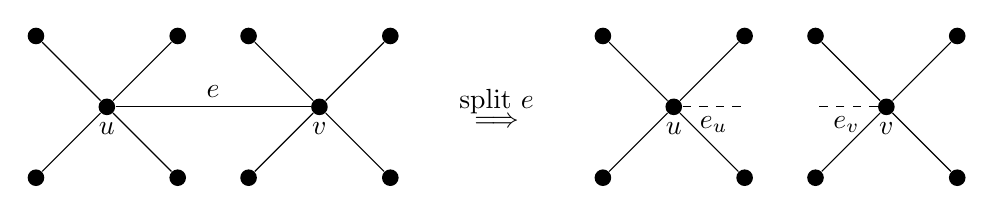
\begin{tikzpicture}[scale=0.9]
        % Left graph
        \node[circle, fill, inner sep=1pt, minimum size=6pt] (lu) at (0, 0) {};
        \node[circle, fill, inner sep=1pt, minimum size=6pt] (lv) at (3, 0) {};
        \node[circle, fill, inner sep=1pt, minimum size=6pt] (l1) at (-1, 1) {};
        \node[circle, fill, inner sep=1pt, minimum size=6pt] (l2) at (-1, -1) {};
        \node[circle, fill, inner sep=1pt, minimum size=6pt] (l3) at (1, 1) {};
        \node[circle, fill, inner sep=1pt, minimum size=6pt] (l4) at (1, -1) {};
        \node[circle, fill, inner sep=1pt, minimum size=6pt] (l5) at (4, 1) {};
        \node[circle, fill, inner sep=1pt, minimum size=6pt] (l6) at (4, -1) {};
        \node[circle, fill, inner sep=1pt, minimum size=6pt] (l7) at (2, 1) {};
        \node[circle, fill, inner sep=1pt, minimum size=6pt] (l8) at (2, -1) {};
    
        \draw (lu) -- (l1);
        \draw (lu) -- (l2);
        \draw (lu) -- (l3);
        \draw (lu) -- (l4);
        \draw (lu) -- (lv) node[midway, above] {$e$};
        \draw (lv) -- (l5);
        \draw (lv) -- (l6);
        \draw (lv) -- (l7);
        \draw (lv) -- (l8);

        \node at (0, -0.3) {$u$};
        \node at (3, -0.3) {$v$};

        % Arrow
        \node at (5.5, 0) {$\stackrel{\mbox{split $e$}}{\Longrightarrow}$};
    
        % Right graph (left part)
        \node[circle, fill, inner sep=1pt, minimum size=6pt] (ru1) at (8, 0) {};
        \node[circle, fill, inner sep=1pt, minimum size=6pt] (r1) at (7, 1) {};
        \node[circle, fill, inner sep=1pt, minimum size=6pt] (r2) at (7, -1) {};
        \node[circle, fill, inner sep=1pt, minimum size=6pt] (r3) at (9, 1) {};
        \node[circle, fill, inner sep=1pt, minimum size=6pt] (r4) at (9, -1) {};
        % \node[draw, circle, fill=black] (re1) at (7, 0) {};

        \draw (ru1) -- (r1);
        \draw (ru1) -- (r2);
        \draw (ru1) -- (r3);
        \draw (ru1) -- (r4);
        \draw[dashed] (ru1) -- (9, 0) node[midway, below] {$e_u$};

        \node at (8, -0.3) {$u$};
    
        % Right graph (right part)
        \node[circle, fill, inner sep=1pt, minimum size=6pt] (rv1) at (11, 0) {};
        \node[circle, fill, inner sep=1pt, minimum size=6pt] (r5) at (10, 1) {};
        \node[circle, fill, inner sep=1pt, minimum size=6pt] (r6) at (10, -1) {};
        \node[circle, fill, inner sep=1pt, minimum size=6pt] (r7) at (12, 1) {};
        \node[circle, fill, inner sep=1pt, minimum size=6pt] (r8) at (12, -1) {};
        % \node[draw, circle, fill=black] (re2) at (8, 0) {};

        \draw (rv1) -- (r5);
        \draw (rv1) -- (r6);
        \draw (rv1) -- (r7);
        \draw (rv1) -- (r8);
        \draw[dashed] (rv1) -- (10, 0) node[midway, below] {$e_v$};

        \node at (11, -0.3) {$v$};
    \end{tikzpicture}
    \caption{An example of splitting the edge $e = \set{u, v}$. $e_u, e_v$ are the half-edges after splitting $e = \set{u, v}$.}
    \label{fig:splitting-edge}
\end{figure}